\documentclass[UTF8,fontset=fandol]{ctexart}
\usepackage[a4paper,margin=23mm]{geometry}
\usepackage{graphicx}
\usepackage[hidelinks]{hyperref}
\setlength{\parindent}{0pt}
\title{XeSINE-Net 项目组织示例}
\author{AI-Native Researchers}
\date{}
\begin{document}
\maketitle
项目首页连接当前研究接力、文献与进展及下一步。阶段索引按编号列出判断页和证据页，稿件和汇报从对应阶段页取得图表和来源。

\begin{figure}[ht]
  \centering
  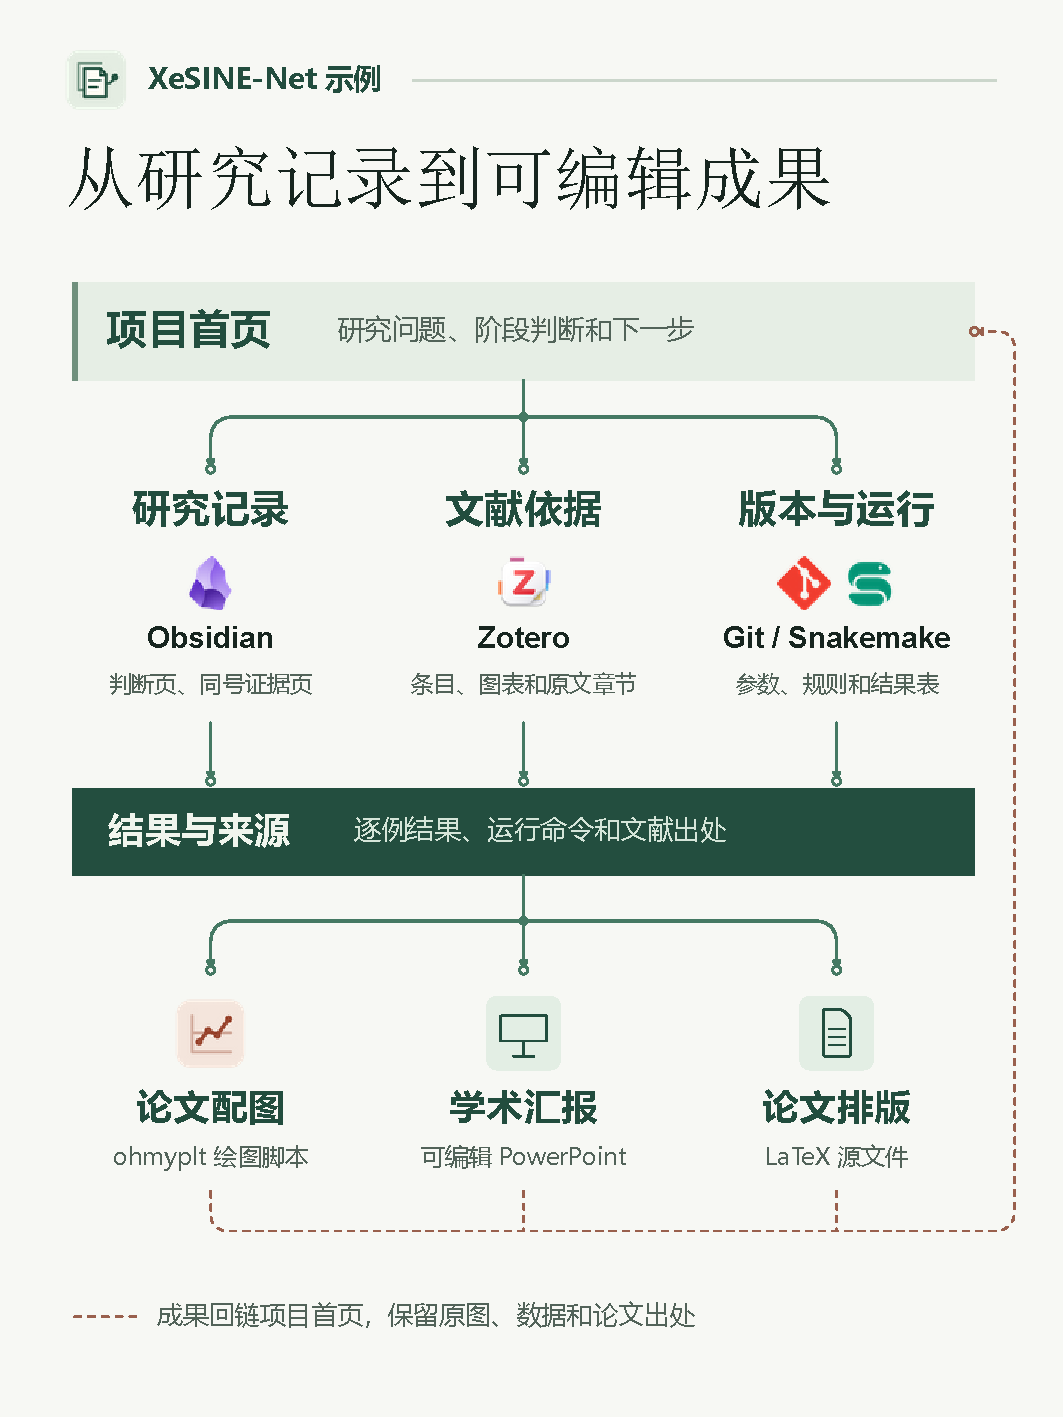
\includegraphics[height=144mm]{../figures/workflow.pdf}
  \caption{从项目首页组织文献、阶段工作和交付文件。}
  \label{fig:workflow}
\end{figure}

图~\ref{fig:workflow} 的绘制方法沿用 ohmyplt 的流程与示意图规范\cite{ohmyplt}。
\begin{thebibliography}{1}
\bibitem{ohmyplt} ohmyplt 科研绘图技能．\url{https://github.com/Lee-Eee-Eee/ohmyplt}.
\end{thebibliography}
\end{document}
